\section{Análisis de resultados}\label{sec:resultados}
El script que se desarrolló se dividió en secciones para alberga la solución de cada uno de los requerimientos del proyecto y cada uno de los resultados gráficos se presentan en una última sección para facilitar la comparación, si es necesaria. Cada sección contiene los parámetros necesarios para las funciones usadas y cada una explicada con comentarios de lo que realiza.

Inicialmente se construyeron los filtros pensando en la posibilidad de poder modificar cualquiera de sus parámetros con el fin de simular un comportamiento similar al diagrama de bloques descrito en la sección~\ref{sec:metodologia} (metodología). Luego de ese proceso el siguiente paso en la secuencia del script se filtra la función con los filtros diseñados y se retorna al dominio del tiempo para observar los resultados.

\subsection{Desarrollo del objetivo clave 1--Aumento del ancho de la banda de paso}
Para el análisis de este objetivo se llevo acabo uno de los escenarios planteados anteriormente, el cual consiste en aumentar el ancho de la banda de paso del pulso rectangular. Como se considero tener los parámetros con la posibilidad de ser variados se aumento dicho parámetro encargado de aumentar el ancho del pulso, significativamente más grande que el ancho de la respuesta en frecuencia de la señal planteada. Se obtuvieron los siguientes resultados.

\begin{figure}[H]
	\centering
	\begin{subfigure}[b]{0.48\linewidth}
		\includegraphics[width=\linewidth]{img/SeñalFiltroIdealF}
		\caption{\scriptsize Respuesta en frecuencia del filtrado.}
		\label{subfig:aumentoFrecuencia}
	\end{subfigure}
	\begin{subfigure}[b]{0.48\linewidth}
		\includegraphics[width=\linewidth]{img/SeñalFiltroIdealT}
		\caption{\scriptsize En el dominio del tiempo.}
		\label{subfig:aumentoTiempo}
	\end{subfigure}
	\vspace{-3mm}
	\caption{\scriptsize Resultados de filtrar la señal original con un filtro ideal pasa-bajas.}
	\label{fig:aumento}
	\vspace{-5mm}
\end{figure}

La gráfica~\ref{subfig:aumentoFrecuencia} muestra como el filtro ideal realiza atenuación a las componentes que quedan por fuera de este y como el ancho de la banda pasante es lo suficientemente grande, las componentes de la señal original pasan por el filtro en su gran mayoría obteniendo en el tiempo una señal bien definida como se muestra en la figura~\ref{subfig:aumentoTiempo}, además permite percibir de que señal se trata.


\subsection{Desarrollo del objetivo clave 2--Disminución del ancho de la banda de paso}
Así como en el anterior objetivo clave se realizó un escenario para apreciar el comportamiento de la señal al filtrarla con un filtro ideal, pero esta vez con banda de paso bastante reducida (1/5 veces el ancho de banda original). La reducción que se aplicó en este caso se consideró que fuera bastante más pequeña para apreciar sus efectos:

\begin{figure}[H]
	\centering
	\begin{subfigure}[b]{0.48\linewidth}
		\includegraphics[width=\linewidth]{img/SeñalFiltroTrapezoidalT}
		\caption{\scriptsize Respuesta en frecuencia del filtrado.}
		\label{subfig:disminucionFrecuencia}
	\end{subfigure}
	\begin{subfigure}[b]{0.48\linewidth}
		\includegraphics[width=\linewidth]{img/SeñalFiltroTrapezoidalF}
		\caption{\scriptsize En el dominio del tiempo.}
		\label{subfig:disminucionTiempo}
	\end{subfigure}
	\vspace{-3mm}
	\caption{\scriptsize Resultados de filtrar la señal original con un filtro ideal.}
	\label{fig:disminucion}
	\vspace{-5mm}
\end{figure}

Se observa que en la figura~\ref{subfig:disminucionFrecuencia} la respuesta del filtrado está muy atenuada por lo que es evidente que sus componentes armónicas se disminuyeron considerablemente, esto se denota en la figura~\ref{subfig:disminucionTiempo} donde la definición de la señal es muy pobre. Sin embargo, con estos dos anteriores resultados se evidencia que la cantidad de armónicos que no son atenuados por el filtro van a depender del ancho de la banda de paso de este.
\subsection{Desarrollo del objetivo clave 3--Análisis de la respuesta del filtro trapezoidal comparado con el filtro ideal}

En los anteriores objetivos se evidenció la respuesta del filtro ideal en diferentes escenarios de ancho de banda. El filtro trapezoidal, se diferencia del filtro ideal en que sus bandas de transición no se presentan como un escalón entre la banda pasante y la banda de rechazo, sino que por el contrario, la atenuación entre estas bandas se presenta de forma gradual siguiendo la forma de una pendiente lineal.

La construcción de este filtro se realizó partiendo de dos funciones ``sinc'' con parámetros variables multiplicadas en el tiempo. Estos parámetros permiten variar los anchos de banda pasante y de transición en el dominio de la frecuencia, como es requerido por el proyecto.

\begin{figure}[H]
	\centering
	\begin{subfigure}[b]{0.48\linewidth}
		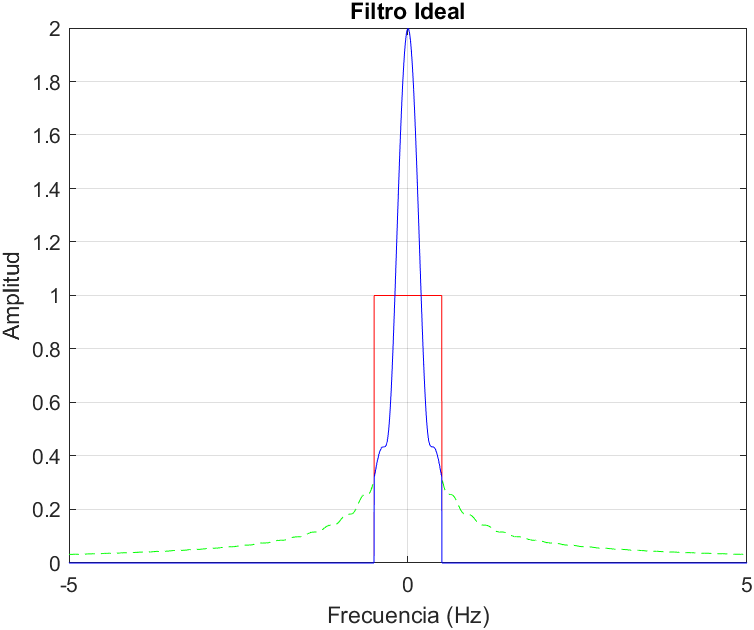
\includegraphics[width=\linewidth]{img/FIdeal}
		\caption{\scriptsize Respuesta en frecuencia del filtro ideal.}
		\label{subfig:frecuenciaIdeal}
	\end{subfigure}
	\begin{subfigure}[b]{0.48\linewidth}
		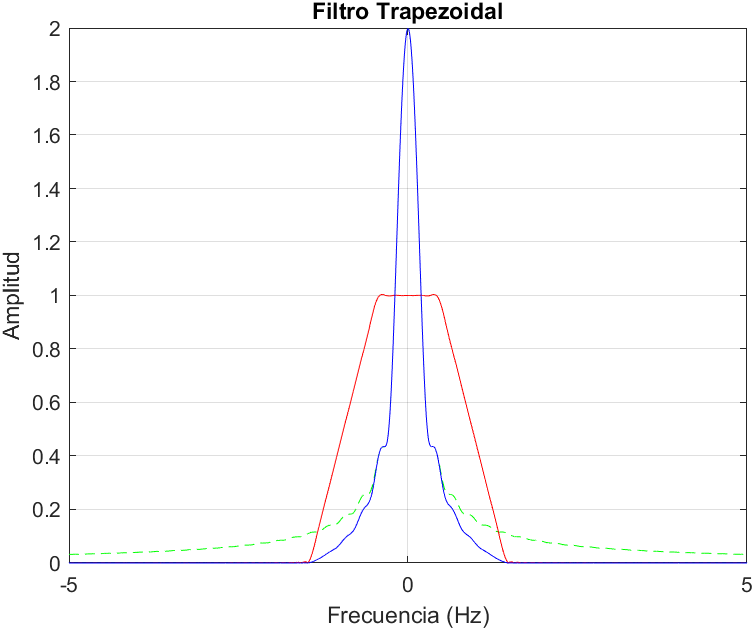
\includegraphics[width=\linewidth]{img/FTrap}
		\caption{\scriptsize Respuesta en frecuencia del filtro trapezoidal.}
		\label{subfig:frecuenciaTrapezoidal}
	\end{subfigure}
	\vspace{-3mm}
	\caption{\scriptsize Comparación de espectros de magnitud donde se evidencian las diferencias en la banda de transición.}
	\label{fig:comparacion}
	\vspace{-5mm}
\end{figure}

En las imágenes anteriores se puede apreciar que las bandas de transición del filtro trapezoidal atenúan menos que en el caso de el filtro ideal, sin embargo al filtrar una señal con un filtro que contiene bandas de transición de cualquier forma, sus componentes armónicas no van a tener el mismo comportamiento que al operar con las componentes de la banda de paso. Ese efecto que se observa en la señal se denomina distorsión lineal.

\subsection{Desarrollo del objetivo clave 4--Análisis del teorema de Rayleigh}
Para el desarrollo de este objetivo, se aplico el teorema de Rayleigh tanto a la señales filtradas y no filtradas tanto en el dominio del tiempo, como en el dominio de la frecuencia. Se tomaron 6 ventanas diferentes de filtrado tanto para el filtro ideal como para el filtro trapezoidal, tomando en cuenta también un escenario donde no se modifica la ventana constante del filtro trapezoidal (a 1 Hz) y se cambia el ancho de sus rampas, todo esto con el objetivo de observar los efectos sobre la energía de la señal al filtrarla. A continuación se presenta una tabla con los resultados:

\begin{figure}[H]
	\centering
	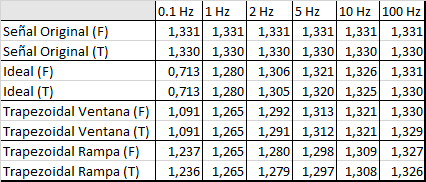
\includegraphics[width=0.7\linewidth]{img/Rayleigh}
	\vspace{-3mm}
	\caption{\scriptsize Tabla de resultados del teorema de Rayleigh.}
	\label{fig:Rayleigh}
	\vspace{-5mm}
\end{figure}

De los resultados obtenidos se puede apreciar que en todos los casos se evidenció el cumplimiento de la igualdad de Rayleigh, por que las magnitud de la densidad espectral de energía en tiempo (T) y frecuencia (F) para cada caso son iguales. Se evidencia un margen de error en la tercera cifra decimal debido a que los cálculos numéricos de las integrales se realizaron con la función ``trapz'', esto debido a la conveniencia de la misma en la estructura del código desarrollado.
Se observa que a menor ancho de banda pasante del filtro, se tiene menor densidad espectral de energía en cada caso, tal como es esperado debido a que un filtro es un sistema que modifica la señal, eliminando componentes espectrales de la misma. Estas componentes eliminadas explican la disminución en magnitud de la densidad espectral de energía con respecto a la señal original.
Al tener una señal de entrada de muy baja frecuencia, se hace evidente que el mayor efecto de filtrado se presenta al introducir la señal a los filtros con ancho de banda pasante menor a 1 Hz. A partir de 1 Hz el efecto del filtrado con respecto a la D.E.E. es menor al 5 por ciento con respecto a la D.E.E. de la señal original.

\begin{figure}[H]
	\centering
	\begin{subfigure}[b]{0.48\linewidth}
		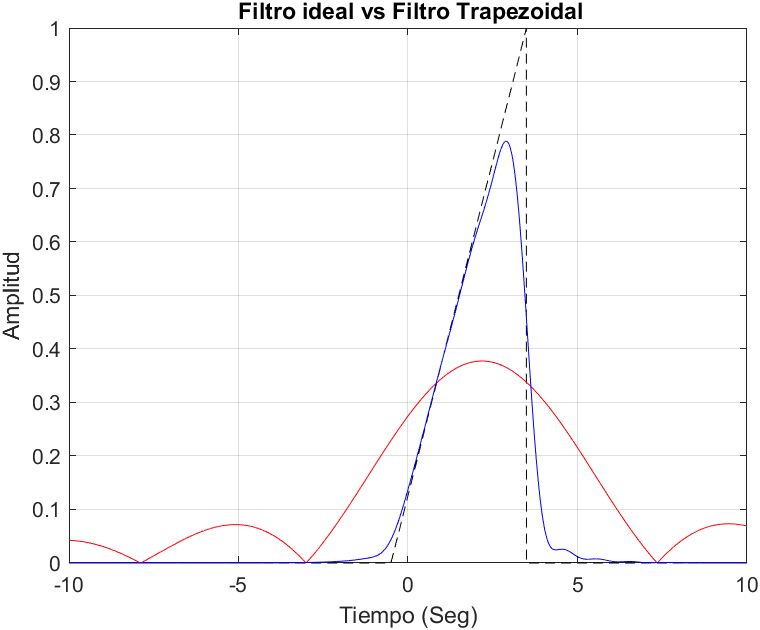
\includegraphics[width=\linewidth]{img/0-1Hz}
		\caption{\scriptsize Respuesta en tiempo del filtrado con 0.1 Hz.}
		\label{subfig:tiempo01}
	\end{subfigure}
	\begin{subfigure}[b]{0.48\linewidth}
		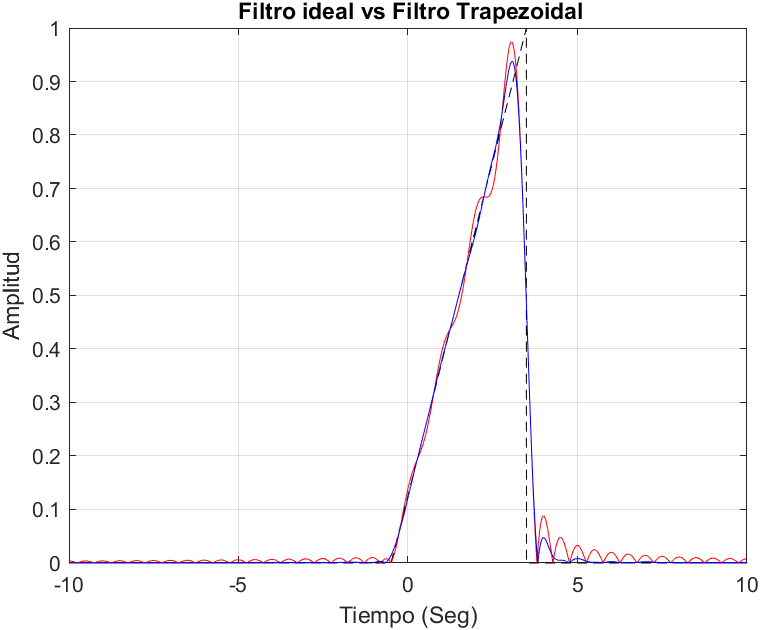
\includegraphics[width=\linewidth]{img/1Hz}
		\caption{\scriptsize Respuesta en tiempo del filtrado con 1 Hz.}
		\label{subfig:tiempo1}
	\end{subfigure}
	\begin{subfigure}[b]{0.48\linewidth}
		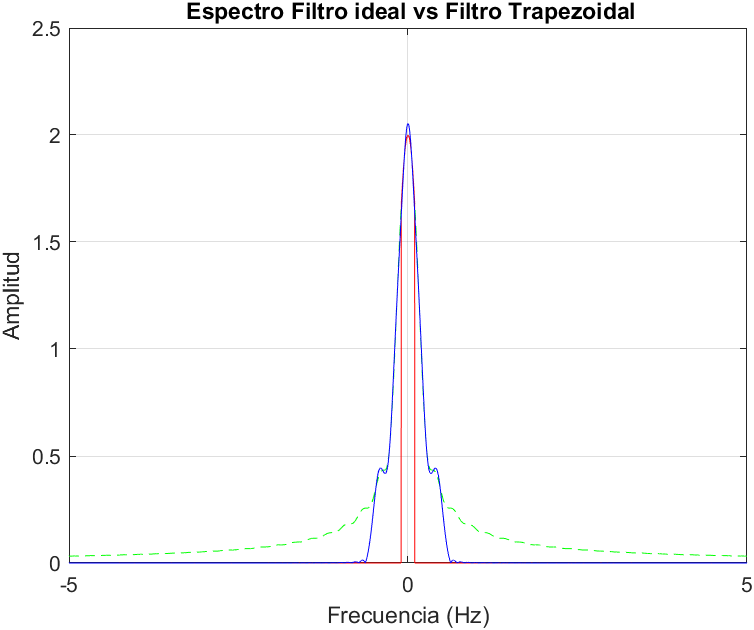
\includegraphics[width=\linewidth]{img/E0-1Hz}
		\caption{\scriptsize Respuesta en frecuencia del filtrado con 0.1 Hz.}
		\label{subfig:frecuencia01}
	\end{subfigure}
	\begin{subfigure}[b]{0.48\linewidth}
		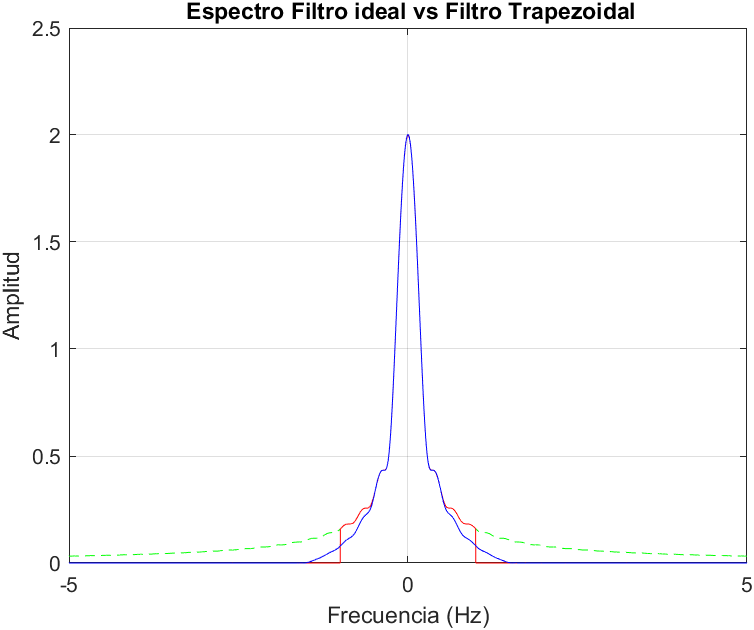
\includegraphics[width=\linewidth]{img/E1Hz}
		\caption{\scriptsize Respuesta en frecuencia del filtrado con 1 Hz.}
		\label{subfig:frecuencia1}
	\end{subfigure}
	\caption{\scriptsize Comparación de Respuestas en tiempo y frecuencia de los filtros vs. Señal original.}
	\label{fig:frecuenciaRayleigh}
	\vspace{-5mm}
\end{figure}

\subsection{Desarrollo del objetivo clave 5--Análisis de la teoría de distorsión lineal}

De acuerdo a la teoría de la distorsión lineal, se evidencian escenarios distintos de acuerdo al tipo de filtro que modifica la señal. Para el caso del filtro ideal, a nivel del espectro de magnitud, se puede apreciar que existe un cambio en el mismo, pero sin la presencia de banda de transición; por este motivo, se puede concluir que aunque se aprecia un cambio en la señal reconstruida debido a la eliminación de armónicos por parte del filtro, este cambio no se puede considerar como distorsión de magnitud en la región del filtro de banda pasante. Cabe resaltar que para obtener una replica exacta de la señal original a la salida del filtro, el ancho de banda del mismo debería ser infinito, es decir un filtro ``pasa todo''.

Por el contrario, para el caso del filtro trapezoidal, se evidencia que en las regiones de banda de transición, los componentes en frecuencia son atenuados de manera no constante, ya que las componentes en frecuencia ubicadas en las partes mas alejadas a la banda de paso son mas atenuadas que las componentes que se encuentran mas cercanas a la banda de paso. Este fenómeno hace que no se cumpla con la condición no-distorsiva:
\begin{equation*}
	y(x)=K\cdot x(t-\tau)
\end{equation*}
Debido a que la señal de salida no se puede expresar como una versión escalar y desfasada de la señal de entrada.

En el caso de considerar el sentido estricto del concepto de distorsión, sin tener en cuenta que el sistema evaluado en esta simulación es un filtro; se puede considerar que al presentar la señal un espectro de magnitud con componentes infinitos, cualquier sistema con una respuesta en frecuencia diferente a ser constante para todas las componentes de frecuencia, introduce distorsión.


\begin{figure}[H]
	\centering
	\begin{subfigure}[b]{0.48\linewidth}
		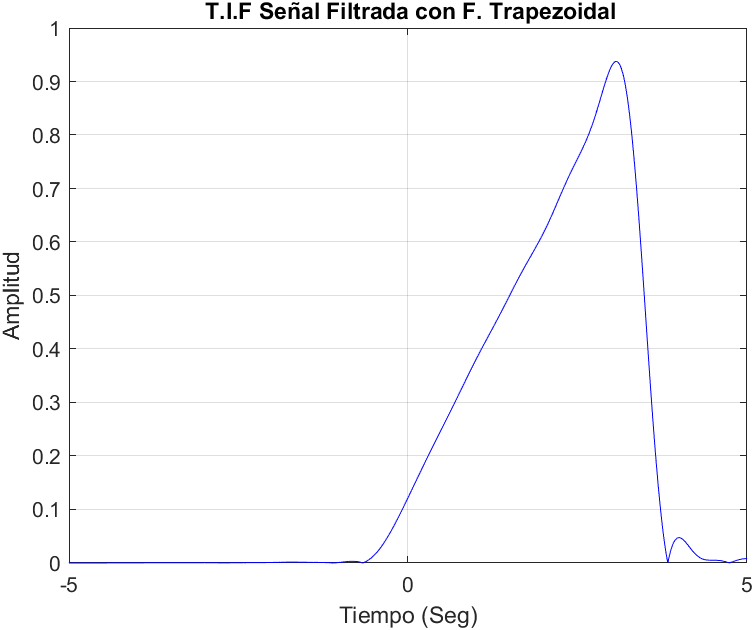
\includegraphics[width=\linewidth]{img/T1Hz}
		\caption{\scriptsize Señal filtrada con el filtro trapezoidal.}
		\label{subfig:distorsionTrapezoidal}
	\end{subfigure}
	\begin{subfigure}[b]{0.48\linewidth}
		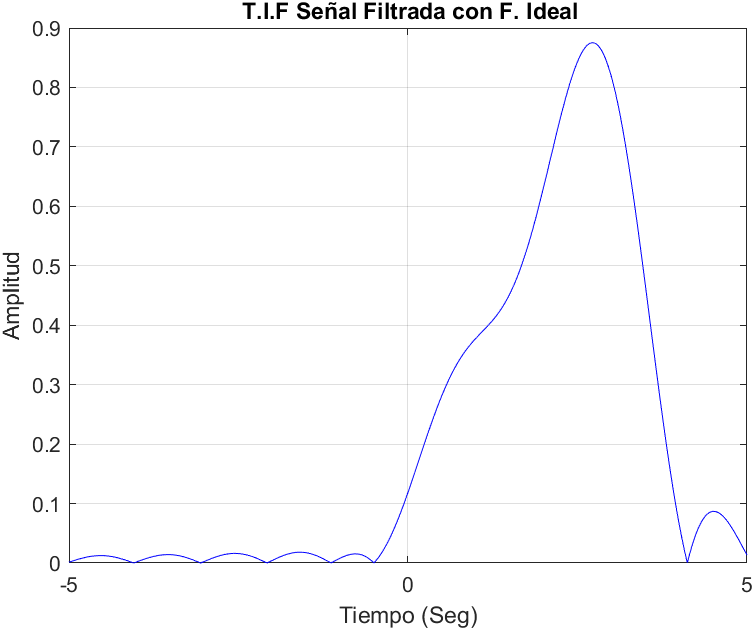
\includegraphics[width=\linewidth]{img/I1Hz}
		\caption{\scriptsize Señal filtrada con el filtro ideal.}
		\label{subfig:distorsionIdeal}
	\end{subfigure}
	\caption{\scriptsize Resultados de filtrar la señal original con un filtro trapezoidal y con un filtro ideal.}
	\label{fig:distorsion}
	\vspace{-5mm}
\end{figure}

las figuras~\ref{subfig:distorsionTrapezoidal} y~\ref{subfig:distorsionIdeal} evidencian la presencia de distorsión al aplicar un filtro que posee bandas en la que su respuesta no es constante. En comparación con la respuesta de aplicar el filtro ideal se ve mejor definido porque este atenúa menos componentes, sin embargo estas componentes que el filtro trapezoidal no atenúa son componentes distorsionadas.
